\documentclass[12pt]{article}

\usepackage[utf8]{inputenc}
\usepackage{geometry}
\geometry{letterpaper, margin=1in}
\usepackage{amsmath}
\usepackage{graphicx}
\usepackage{subcaption}
\usepackage{booktabs}
\usepackage[numbers,super]{natbib}
\usepackage{float}
\usepackage{array}
\usepackage{caption}
\usepackage{hyperref}
\hypersetup{colorlinks=true,linkcolor=black,citecolor=black,urlcolor=blue}
\usepackage{amsmath}
\usepackage{graphicx}
\usepackage{booktabs}
\usepackage[numbers,super]{natbib} % For ACS citation style baseline
\usepackage{hyperref}
\usepackage{fontawesome5} % for using icons
\usepackage[dvipsnames]{xcolor}
\usepackage{textcomp}
\usepackage{pdfpages}
\usepackage{siunitx}
\usepackage{adjustbox}

\begin{document}

\begin{center}
    \Large \textbf{Lab \#6: Fluorescence of Anthracene:}\\[0.2em]
\end{center}
\vspace{0.5em}

\noindent
\begin{minipage}[t]{0.5\textwidth}
    \small
    \textbf{Name:} Yuchen Shi \\
    \textbf{Lab Partner:} Yizhe Dai, Siqi Li \\
    \textbf{Section:} 001
\end{minipage}%
\begin{minipage}[t]{0.5\textwidth}
    \small \raggedleft
    \textbf{Date Performed:} 2026-04-07 \\
    \textbf{Date Submitted:} \today
\end{minipage}
\vspace{1.5em}

\begin{abstract}
Anthracene fluorescence in cyclohexane was measured with a spectrometer to examine vibronic structure and quenching phenomena with ethyl iodide. Emission spectra were recorded at excitation wavelengths of 340 and 325 nm, an excitation spectrum was acquired by monitoring emission at 425 nm. Quenching spectra were measured for 0.050 M, 0.100 M, 0.150 M, and 0.200 M ethyl iodide. Emission and excitation peak spacings showed average apparent vibrational spacings of 1382.561 $\pm$ 16.321 cm$^{-1}$ for $S_0$ and 1427.825 $\pm$ 27.260 cm$^{-1}$ for $S_1$. Four Stern-Volmer fits yielded an average quenching constant of $K_{SV}=18.500 \pm 0.110$ M$^{-1}$ with 95\% confidence interval and an apparent bimolecular quenching constant of $(3.830 \pm 0.023)\times10^9$ M$^{-1}$ s$^{-1}$. The experimental $K_{SV}$ agreed well with literature values of 18.800 and 19.100 M$^{-1}$, differing by 1.596\% and 3.141\%, respectively.
\end{abstract}

\section*{Introduction}
Fluorescence spectroscopy is a useful method for studying how molecules behave after absorbing light. When a molecule absorbs radiation, it can be promoted from the ground electronic state $S_0$ to an excited singlet state. It may then lose part of its energy non-radiatively and return to the ground state by emitting light, which is observed as fluorescence. For aromatic molecules such as anthracene, these electronic transitions are usually accompanied by vibrational structure, so the spectra often show several distinct peaks instead of one broad band. The positions and spacings of these peaks can be used to learn about the vibrational energy levels in the ground and excited states. Anthracene is a good molecule for this experiment because it fluoresces strongly in cyclohexane and its vibronic structure is relatively easy to observe.

Also, an important principle in fluorescence is Kasha’s rule, which states that fluorescence generally occurs from the lowest excited singlet state, even if the molecule is initially excited at a higher energy. Because of this, changing the excitation wavelength is not expected to greatly change the wavelengths of the fluorescence peaks, although the overall intensity may change depending on how strongly the sample absorbs at the chosen excitation wavelength. Comparing the emission spectra obtained at two different excitation wavelengths can therefore show whether the observed behavior is consistent with this rule. In addition, the excitation spectrum and the fluorescence spectrum are expected to have related vibronic structure, and in many cases they show approximate mirror symmetry. This makes it possible to use both spectra together to estimate vibrational level spacings in $S_0$ and $S_1$. Fluorescence can also be reduced by quenching. In this experiment, ethyl iodide was used as a quencher for anthracene in cyclohexane. The quencher provides an additional non-radiative pathway that competes with fluorescence, so the observed emission intensity decreases as quencher concentration increases. For dynamic quenching, this relationship is described by the Stern–Volmer equation
\begin{equation}
\frac{F_0}{F} = 1 + K_{SV}[Q] = 1 + \tau_0 k_q [Q]
\label{eq:sv}
\end{equation}
where $F_0$ is the fluorescence intensity without quencher, $F$ is the intensity with quencher, $[Q]$ is the quencher concentration, $K
_{SV}$ is the Stern–Volmer constant, $\tau_0$ is the fluorescence lifetime in the absence of quencher, and $k_q$ is the apparent bimolecular quenching constant. A plot of $\frac{F_0}{F}$ versus $[Q]$ should therefore be linear if the quenching is well described by the Stern–Volmer model.

The purpose of this experiment was to record the fluorescence and excitation spectra of anthracene, compare the spectra obtained under different excitation conditions, and examine the quenching effect of ethyl iodide. From the spectral peaks, vibronic energy level spacings were estimated, and from the quenching data, Stern–Volmer plots were constructed to determine the experimental quenching constant. The experimental results were then compared with literature values reported for the anthracene–ethyl iodide–cyclohexane system.

\section*{Experimental}
A quartz fluorescence cuvette was filled with the stock anthracene solution in cyclohexane, approximately $1.7\times10^{-5}$ M concentration. Emission spectra were first recorded from 370 to 480 nm with excitation fixed at 340 nm. A second emission spectrum was recorded under identical conditions except that the excitation wavelength was changed to 325 nm. The two emission spectra were overlaid to compare peak positions and relative intensities.

Next, an excitation spectrum was recorded by fixing the emission wavelength at 425 nm and scanning the excitation wavelength from 300 to 400 nm. The excitation spectrum was then overlaid with the 340 nm emission spectrum to compare their vibronic structure.

For the quenching study, the anthracene solution without quencher was scanned under the same emission conditions used for the 340 nm spectrum. Additional anthracene solutions containing 0.050, 0.100, 0.150, and 0.200 M ethyl iodide were prepared in 25.00 mL volumetric flasks. The required ethyl iodide volumes were 100, 200, 300, and 400 $\mu$L, respectively based on a density of 1.950 g mL$^{-1}$ and molar mass of 155.97 g mol$^{-1}$. Each solution was used to rinse the cuvette before the corresponding fluorescence spectrum was acquired. The quenching analysis was based on the fluorescence spectra for 0.000, 0.050, 0.100, 0.150, and 0.200 M ethyl iodide, where the linear regessions were conducted in Python using Matplotlib\cite{Hunter2007_matplotlib} and Numpy \cite{harris2020array} libraries.

\section*{Results}

\begin{figure}[H]
    \centering
    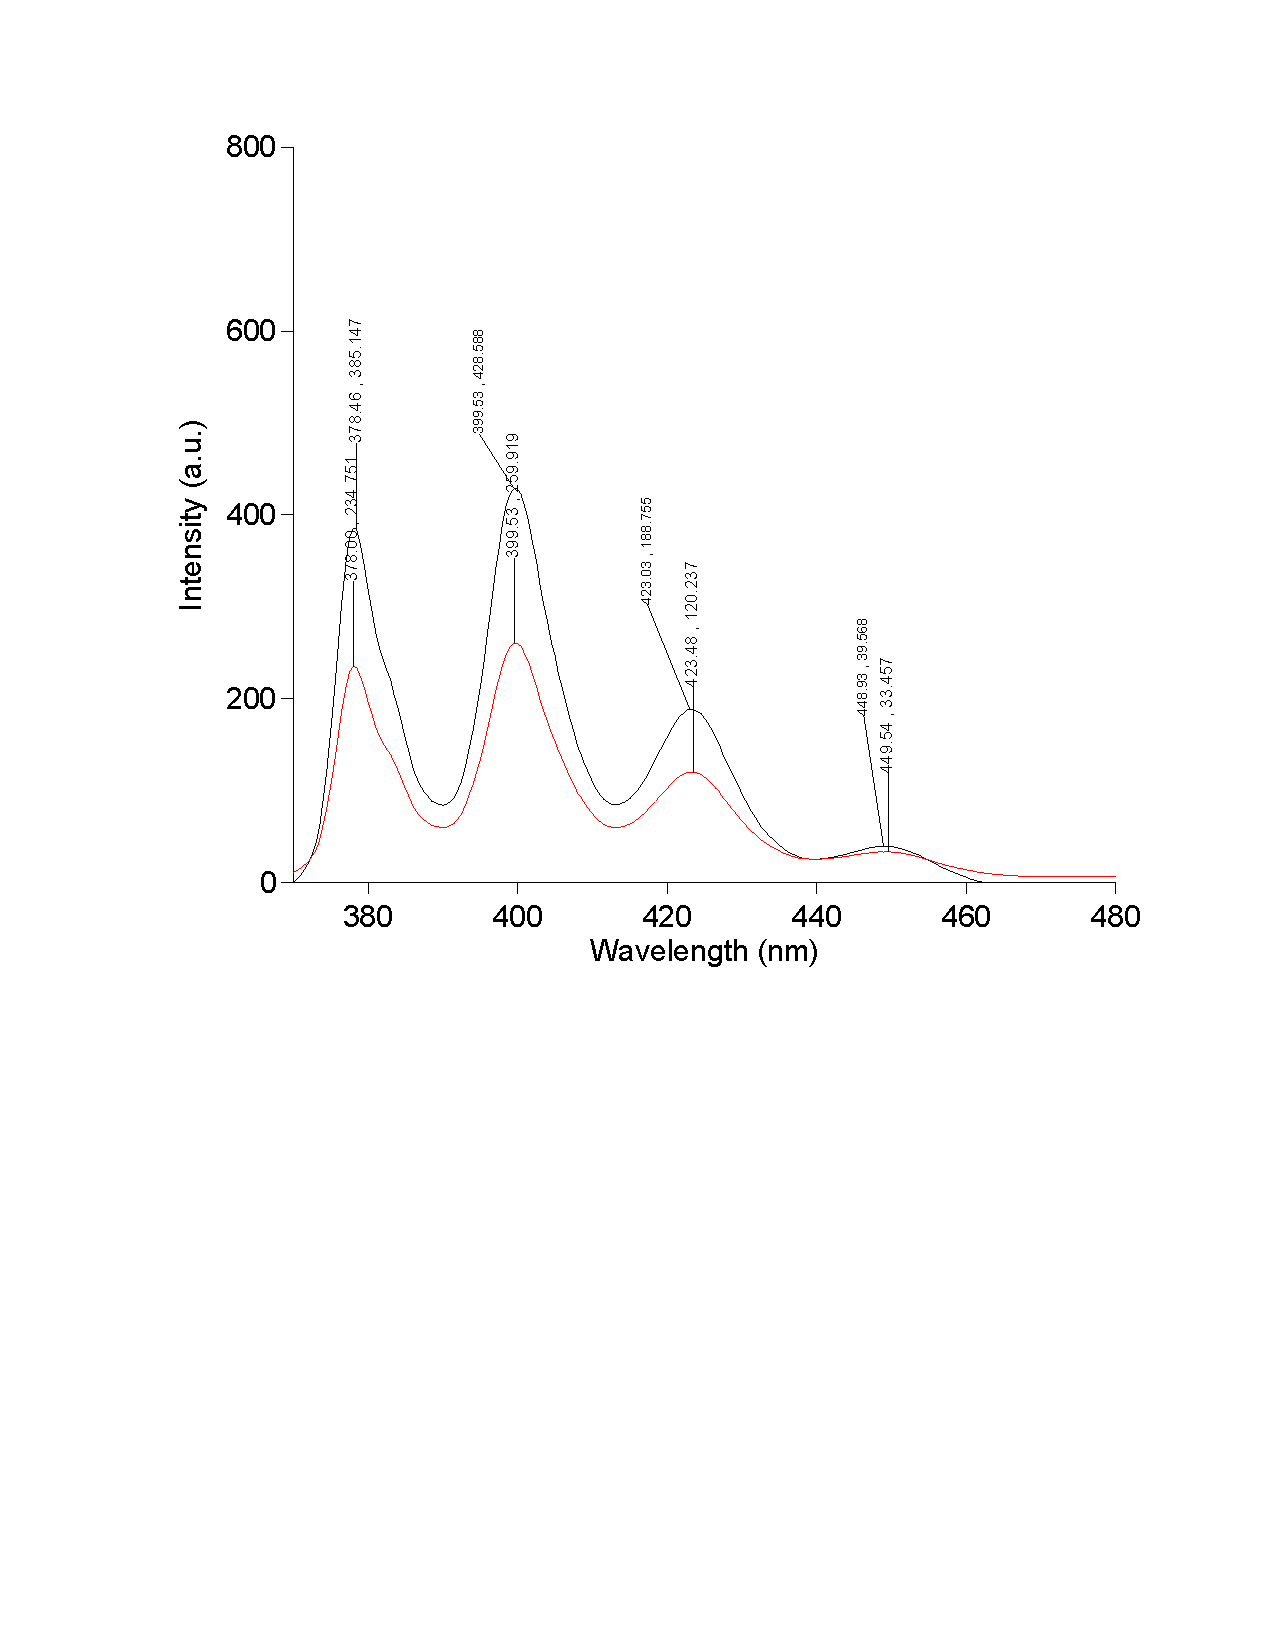
\includegraphics[width=0.6\textwidth]{spectrum/340-325_Excitation.pdf}
    \caption{Overlay of emission spectra recorded with excitation wavelengths of 340 and 325 nm. Peak positions are basically unchanged, while the 325 nm excitation produces lower fluorescence intensity.}
    \label{fig:emissionoverlay}
\end{figure}
\begin{figure}[H]
    \centering
    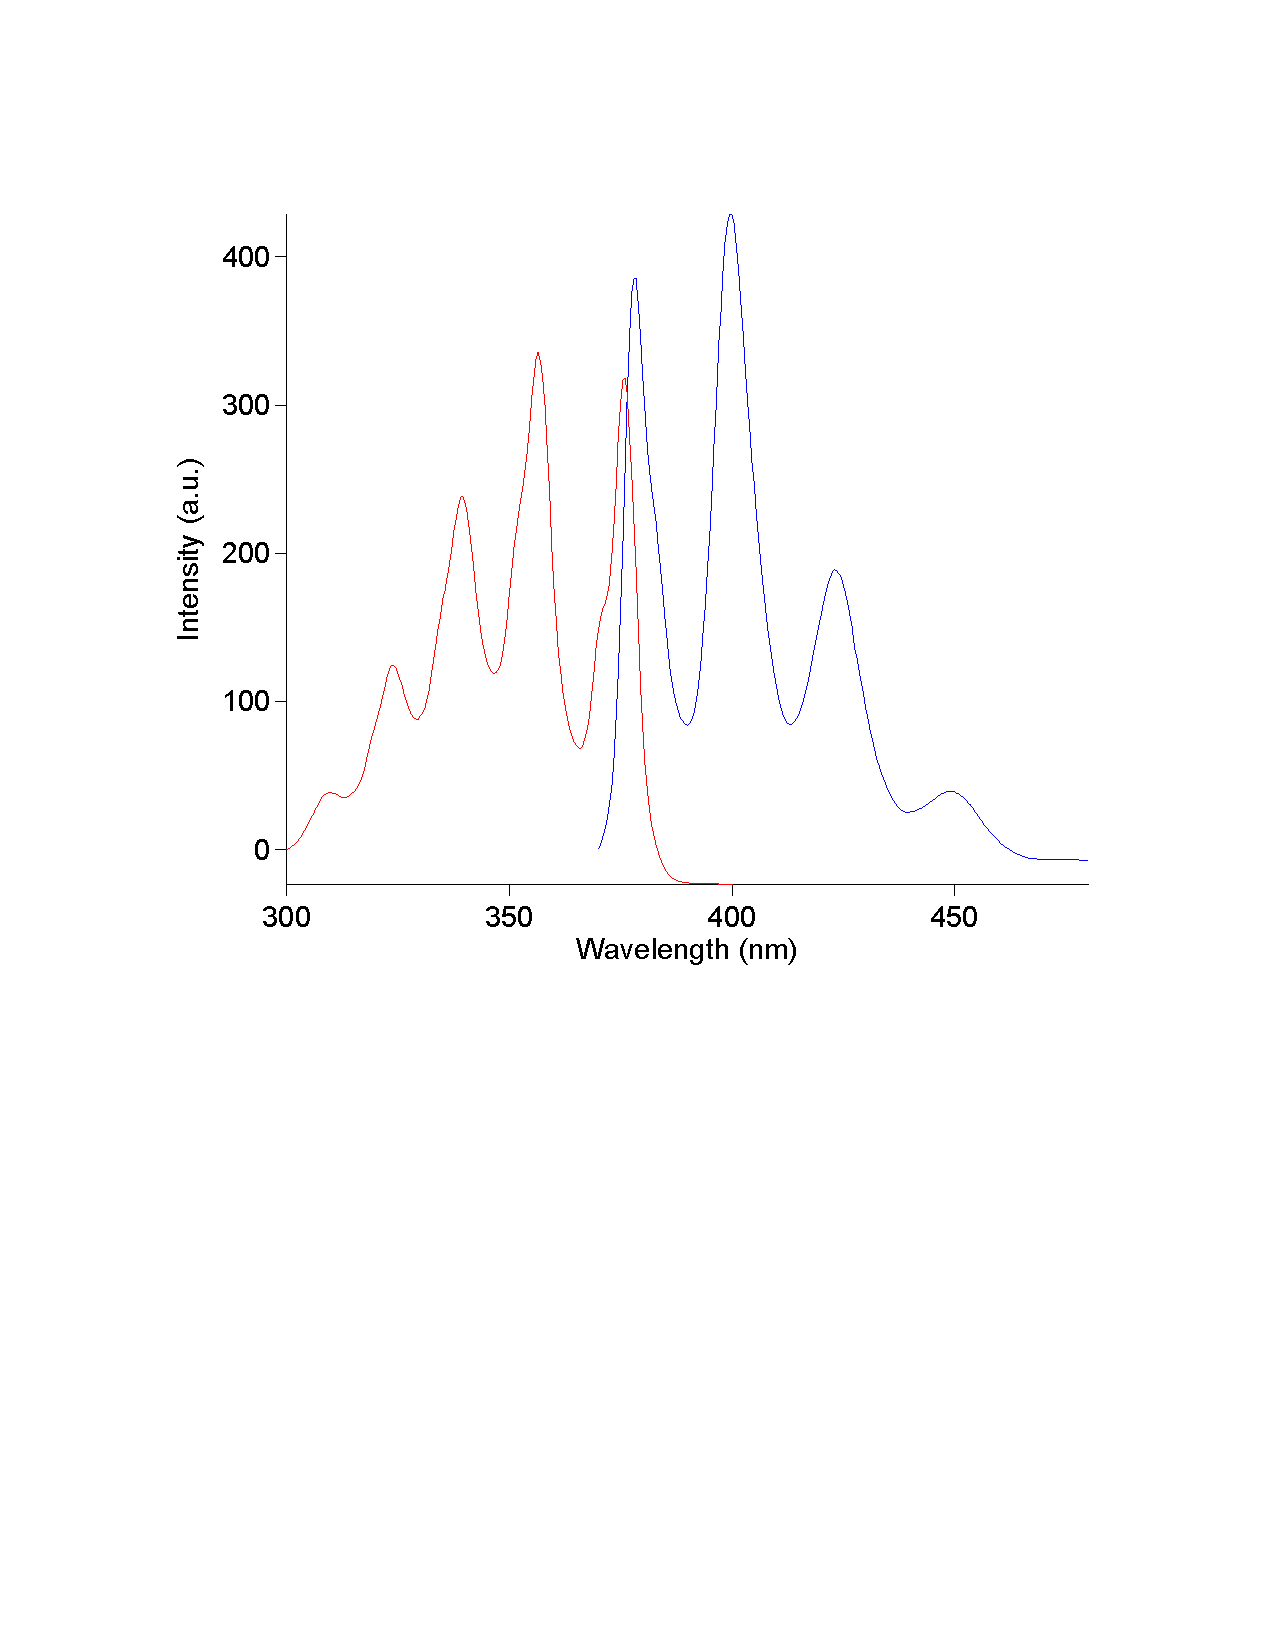
\includegraphics[width=0.62\textwidth]{spectrum/excitation_emission.pdf}
    \caption{Overlay of the excitation spectrum monitored at 425 nm and the 340 nm emission spectrum. }
    \label{fig:excemoverlay}
\end{figure}
The 340 and 325 nm emission spectra showed the same four main vibronic bands around 378, 400, 423, and 449 nm, but the 325 nm spectrum was uniformly weaker. The overlay is shown in Figure~\ref{fig:emissionoverlay}. The excitation spectrum monitored at 425 nm displayed five peaks at 309.530, 324.000, 339.530, 356.460, and 376.000 nm. When overlaid with the 340 nm emission spectrum, it showed the expected complementary vibronic progression (Figure~\ref{fig:excemoverlay}).

Peak positions and intensities from the unquenched emission spectra are summarized in Table~\ref{tab:empeaks}. The differences in peak wavelength between the two excitation conditions were at most 0.610 nm, whereas the intensity ratios $I_{325}/I_{340}$ ranged from 0.607 to 0.846. Thus, changing the excitation wavelength affected the signal magnitude much more than the emission peak positions.

\begin{table}[H]
\centering
\caption{Emission peak positions and intensities for anthracene in cyclohexane.}
\label{tab:empeaks}
\begin{tabular}{cccccc}
\toprule
Peak & $\lambda_{340}$ / nm & $I_{340}$ / a.u. & $\lambda_{325}$ / nm & $I_{325}$ / a.u. & $I_{325}/I_{340}$ \\
\midrule
1 & 378.460 & 385.147 & 378.000 & 234.751 & 0.610 \\
2 & 399.530 & 428.588 & 399.530 & 259.919 & 0.607 \\
3 & 423.030 & 188.755 & 423.480 & 120.237 & 0.637 \\
4 & 448.930 & 39.568  & 449.540 & 33.457  & 0.846 \\
\bottomrule
\end{tabular}
\end{table}

To estimate the apparent vibronic spacings, the measured wavelengths were converted to wavenumbers using $\tilde{\nu} = \frac{10^7}{\lambda\, (\mathrm{nm})}$. For the 340 nm emission spectrum, the four peaks corresponded to 26422.872, 25029.410, 23638.985, and 22275.188 cm$^{-1}$, giving $S_0$ spacings of 1393.462, 1390.424, and 1363.798 cm$^{-1}$. 

For the excitation spectrum, the progression 376.000, 356.460, 339.530, 324.000, and 309.530 nm corresponded to 26595.745, 28053.639, 29452.478, 30864.198, and 32307.046 cm$^{-1}$, giving $S_1$ spacings of 1457.894, 1398.840, 1411.719, and 1442.849 cm$^{-1}$. These values are summarized in Table~\ref{tab:spacing} and visualized in Figure~\ref{fig:energy}.

\begin{table}[H]
\centering
\caption{Vibronic spacings derived from measured emission and excitation peaks. Uncertainties are reported as the sample standard deviation.}
\label{tab:spacing}
\begin{tabular}{lcc}
\toprule
Electronic state & Adjacent spacings / cm$^{-1}$ & Mean spacing / cm$^{-1}$ \\
\midrule
$S_0$ & 1393.462, 1390.424, 1363.798 & 1382.561 $\pm$ 16.321 \\
$S_1$ & 1457.894, 1398.840, 1411.719, 1442.849 & 1427.825 $\pm$ 27.260 \\
\bottomrule
\end{tabular}
\end{table}

\begin{figure}[H]
    \centering
    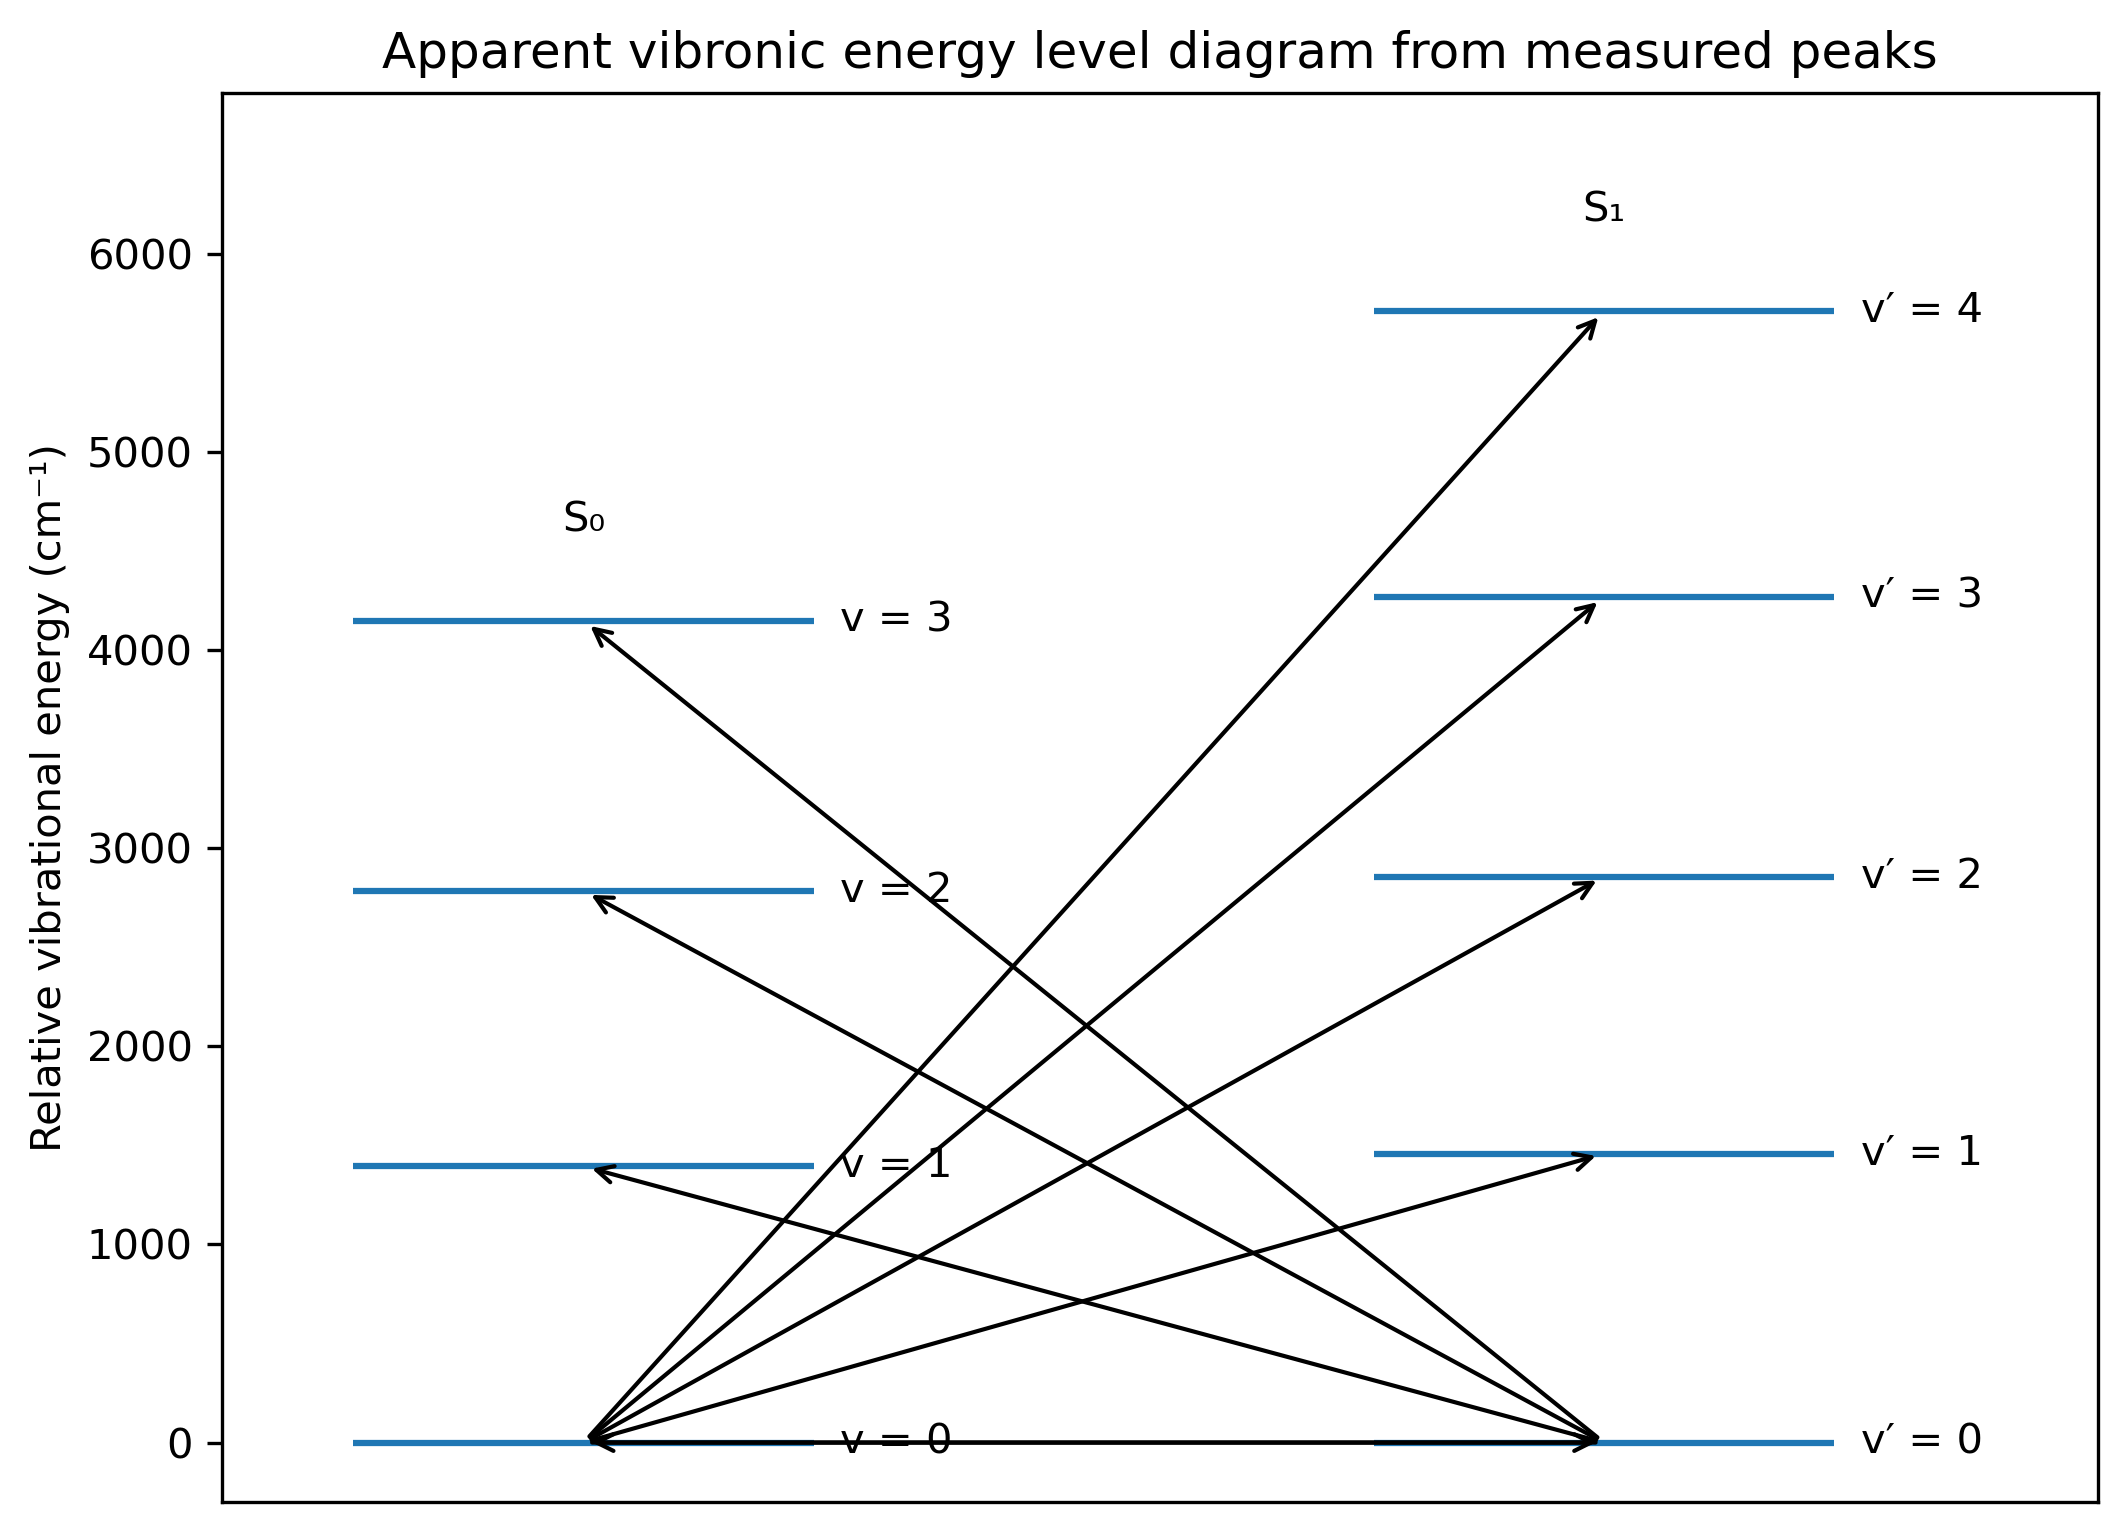
\includegraphics[width=0.72\textwidth]{energy_diagram.png}
    \caption{Apparent vibronic energy level diagram constructed from the measured excitation and emission peak positions.}
    \label{fig:energy}
\end{figure}

The quenching spectra decreased systematically in intensity as ethyl iodide concentration increased, and they preserved an approximately linear Stern-Volmer trend (Figure~\ref{fig:quenchoverlay}). The fluorescence intensities used in the Stern-Volmer analysis are listed in Table~\ref{tab:f0f}. For each emission band, $F_0/F$ was calculated from the unquenched intensity and the corresponding quenched intensity. 

\begin{figure}[H]
    \centering
    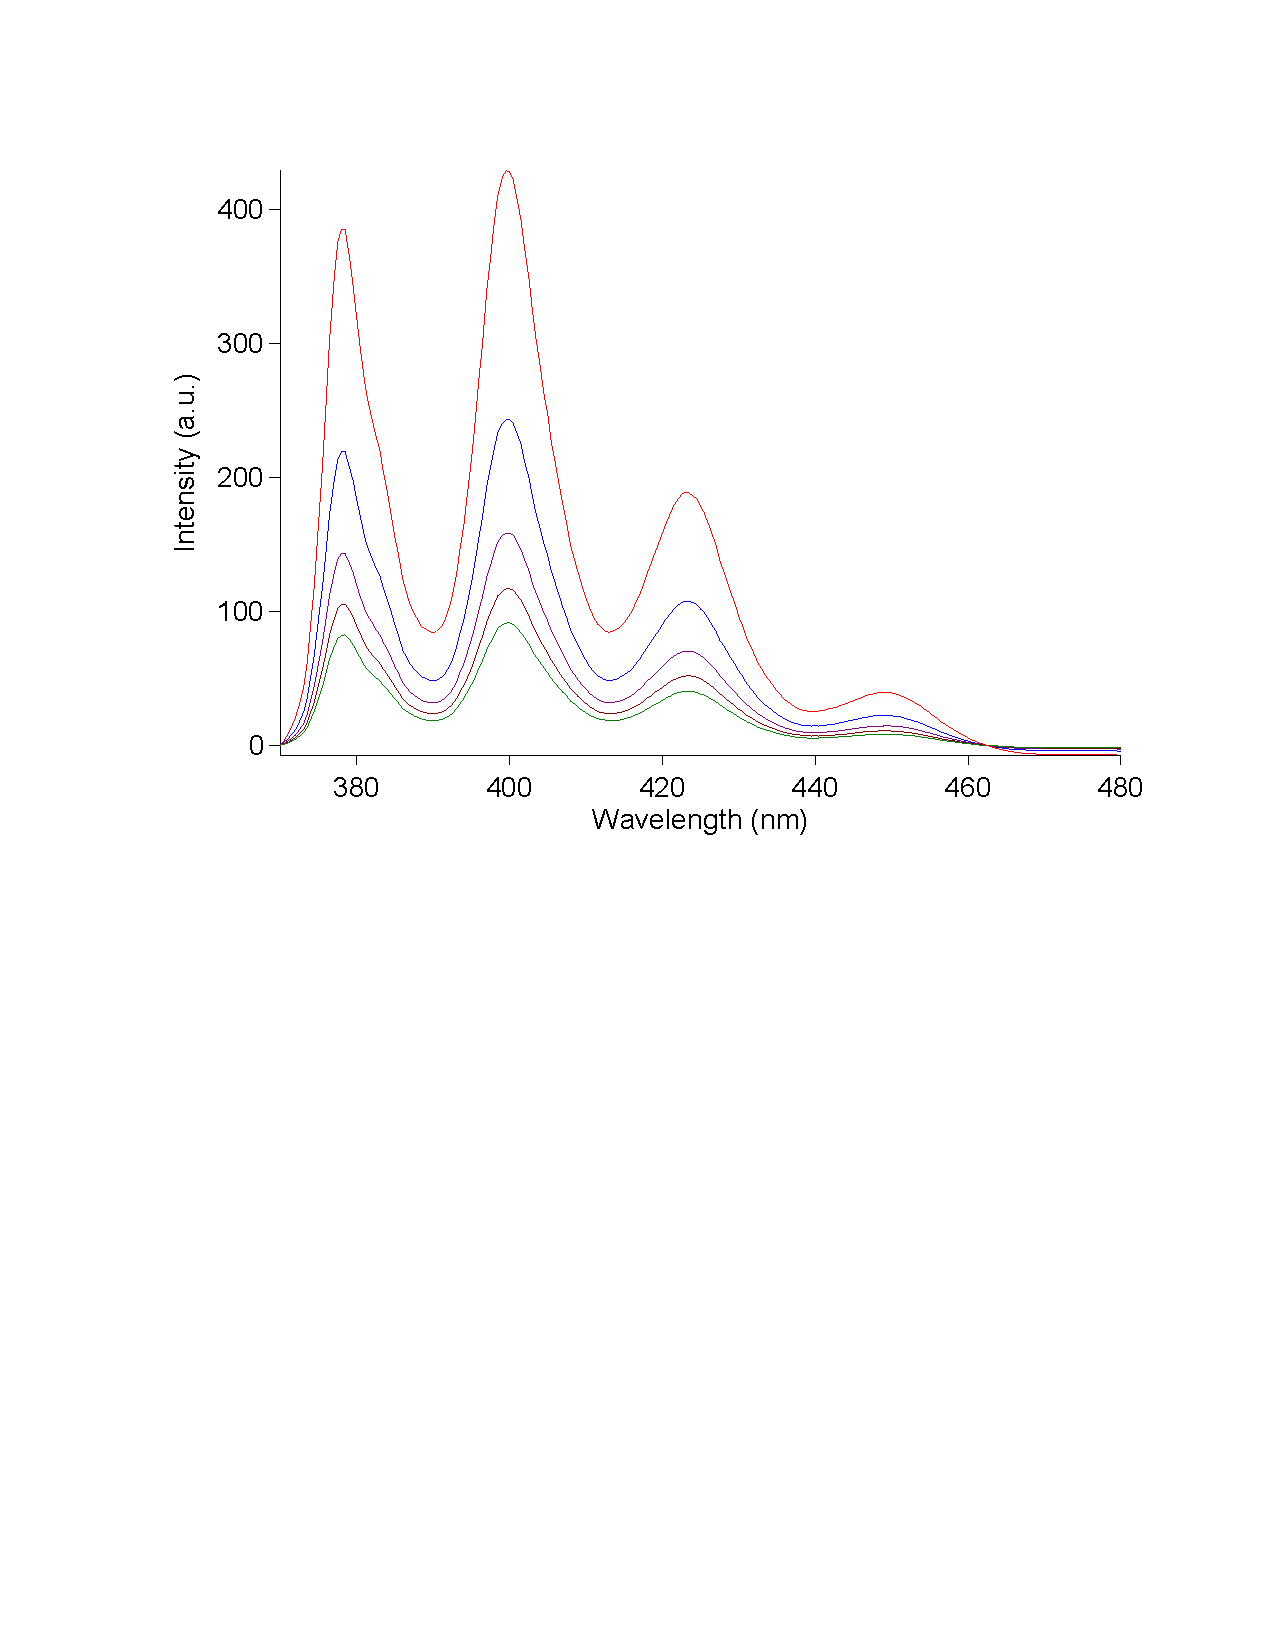
\includegraphics[width=0.76\textwidth]{spectrum/overlay.pdf}
    \caption{Overlay of fluorescence spectra used for the quenching analysis. The five curves are from 0 M, 0.050 M, 0.100 M, 0.150 M, 0.200 M quenchers respectively with decreased peak heights.}
    \label{fig:quenchoverlay}
\end{figure}

\begin{table}[H]
\centering
\caption{Values of $F_0/F$ used in the Stern-Volmer analysis. Quenched peaks were matched to the nearest unquenched emission peak.}
\label{tab:f0f}
\begin{tabular}{cccccc}
\toprule
Peak / nm & $F_0$ & $F_0/F$ at 0.050 M & $F_0/F$ at 0.100 M & $F_0/F$ at 0.150 M & $F_0/F$ at 0.200 M \\
\midrule
378.460 & 385.147 & 1.759 & 2.696 & 3.658 & 4.673 \\
399.530 & 428.588 & 1.764 & 2.710 & 3.670 & 4.685 \\
423.030 & 188.755 & 1.755 & 2.684 & 3.640 & 4.659 \\
448.930 & 39.568  & 1.777 & 2.719 & 3.642 & 4.706 \\
\bottomrule
\end{tabular}
\end{table}

Each Stern-Volmer plot was fit to a straight line of the form
\begin{equation}
y = kx +b
\end{equation}
with $x=[Q]$ and $y=F_0/F$. The uncertainties displayed on the regression plots are the \emph{standard errors} of the fitted slope and intercept. Figure~\ref{fig:svpanel} shows all four regression plots; numerical fit results are summarized in Table~\ref{tab:fits}.

\begin{figure}[H]
    \centering
    \begin{subfigure}[b]{0.48\textwidth}
        \centering
        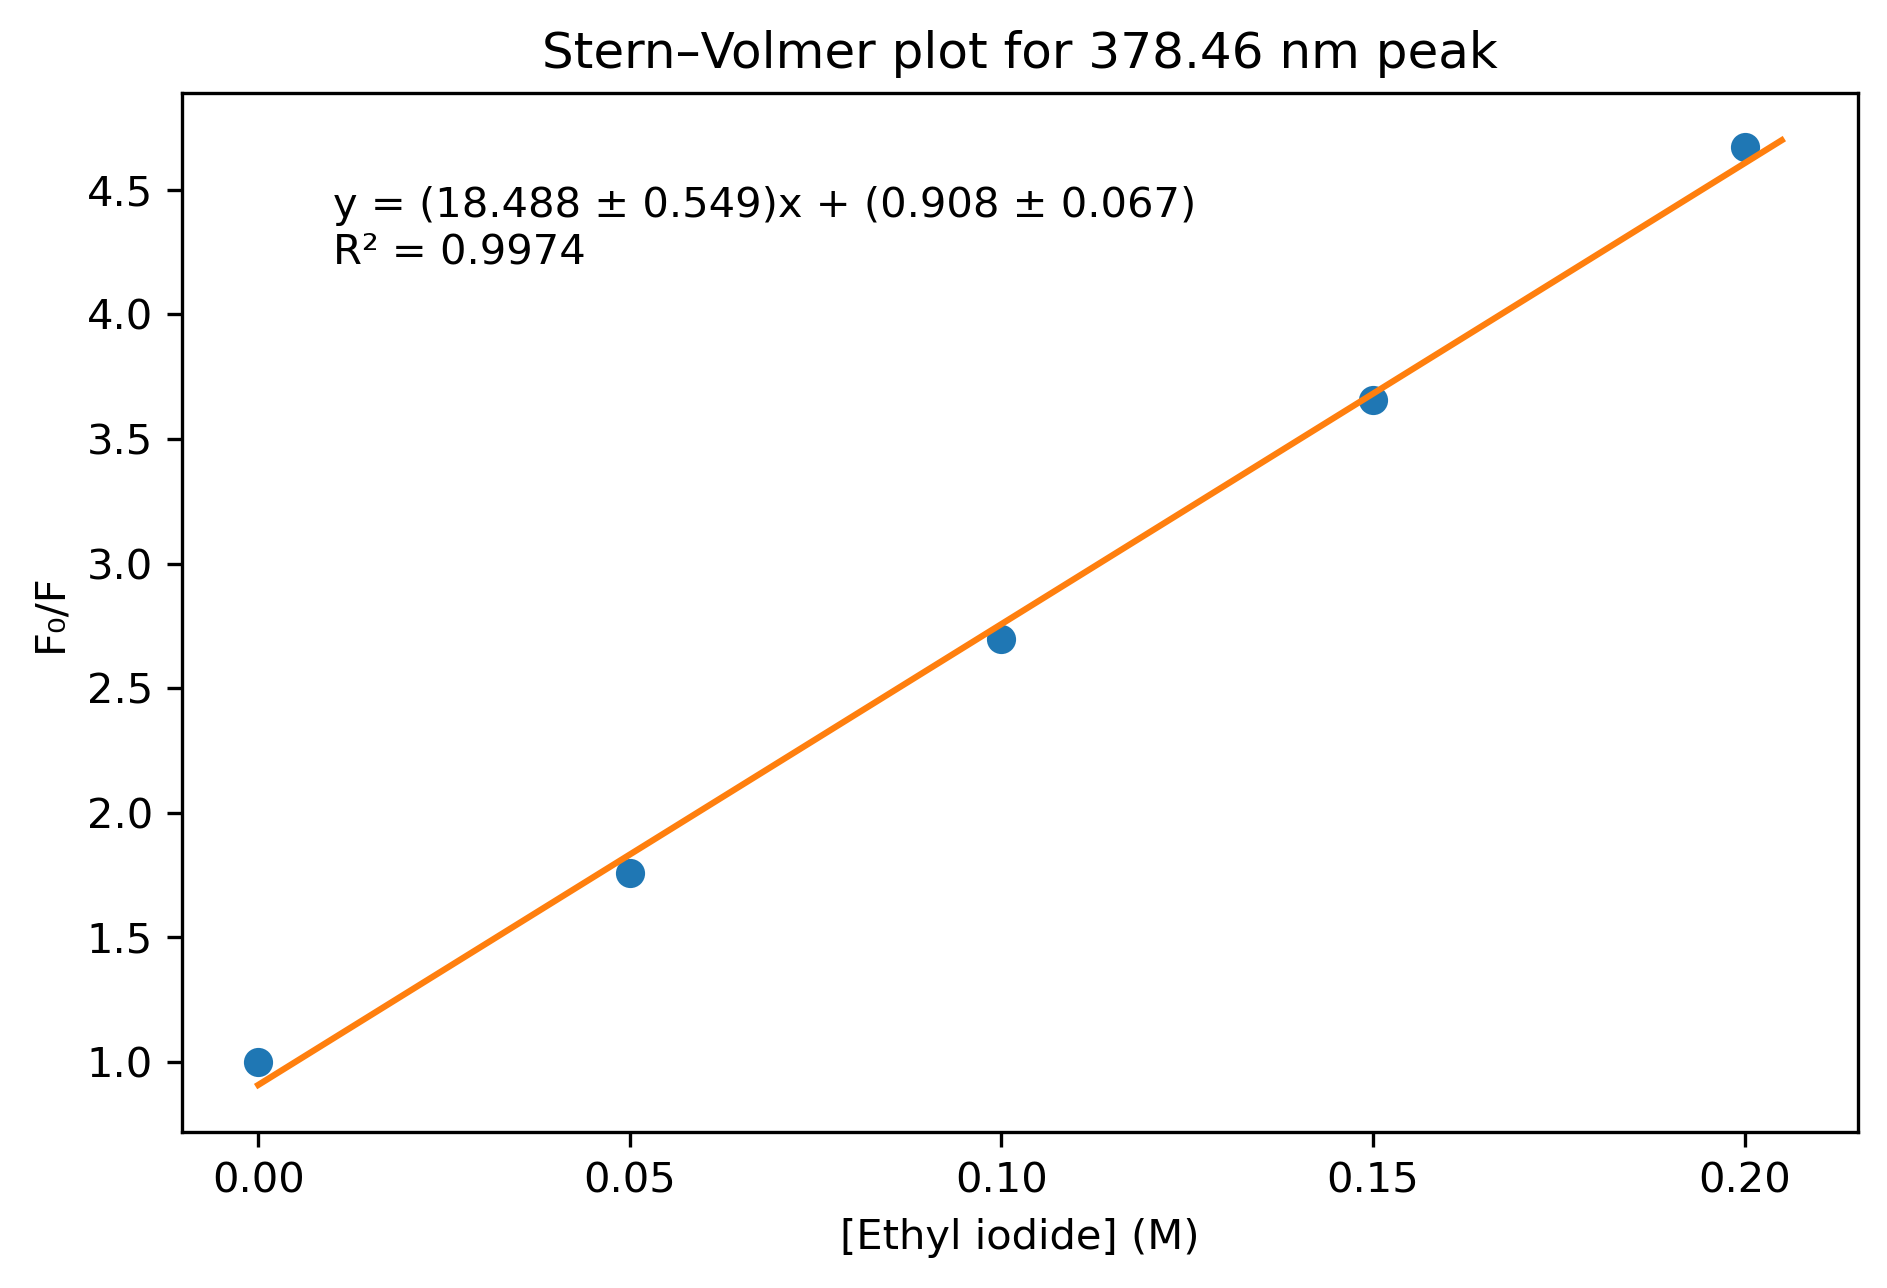
\includegraphics[width=\textwidth]{regression/stern_volmer_378p46nm.png}
        \caption{Linear Regression for Peak 1}
        \label{fig:sv_peak1}
    \end{subfigure}
    \hfill
    \begin{subfigure}[b]{0.48\textwidth}
        \centering
        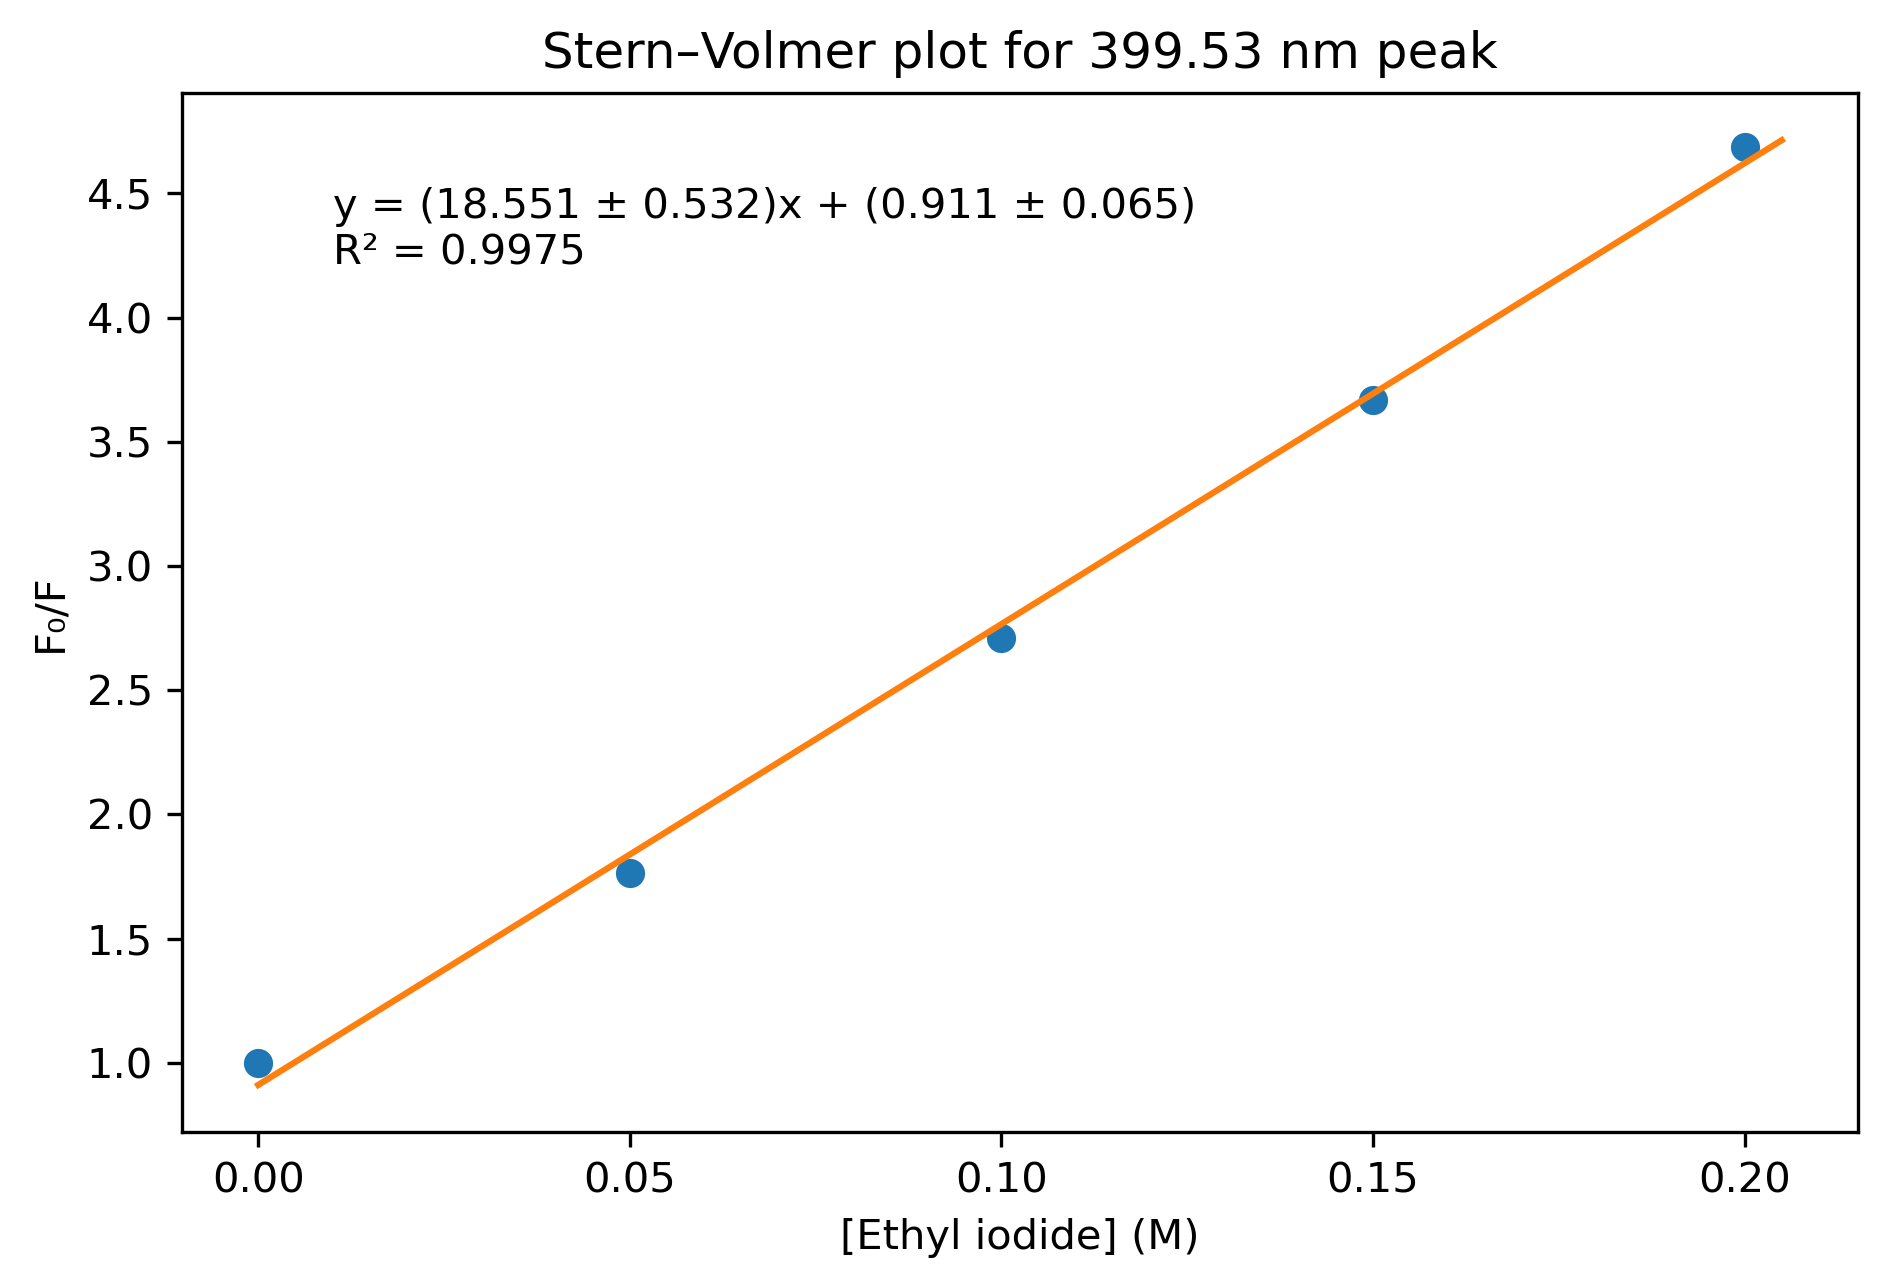
\includegraphics[width=\textwidth]{regression/stern_volmer_399p53nm.png}
        \caption{Linear Regression for Peak 2}
        \label{fig:sv_peak2}
    \end{subfigure}
    \vspace{1em} 
    \begin{subfigure}[b]{0.48\textwidth}
        \centering
        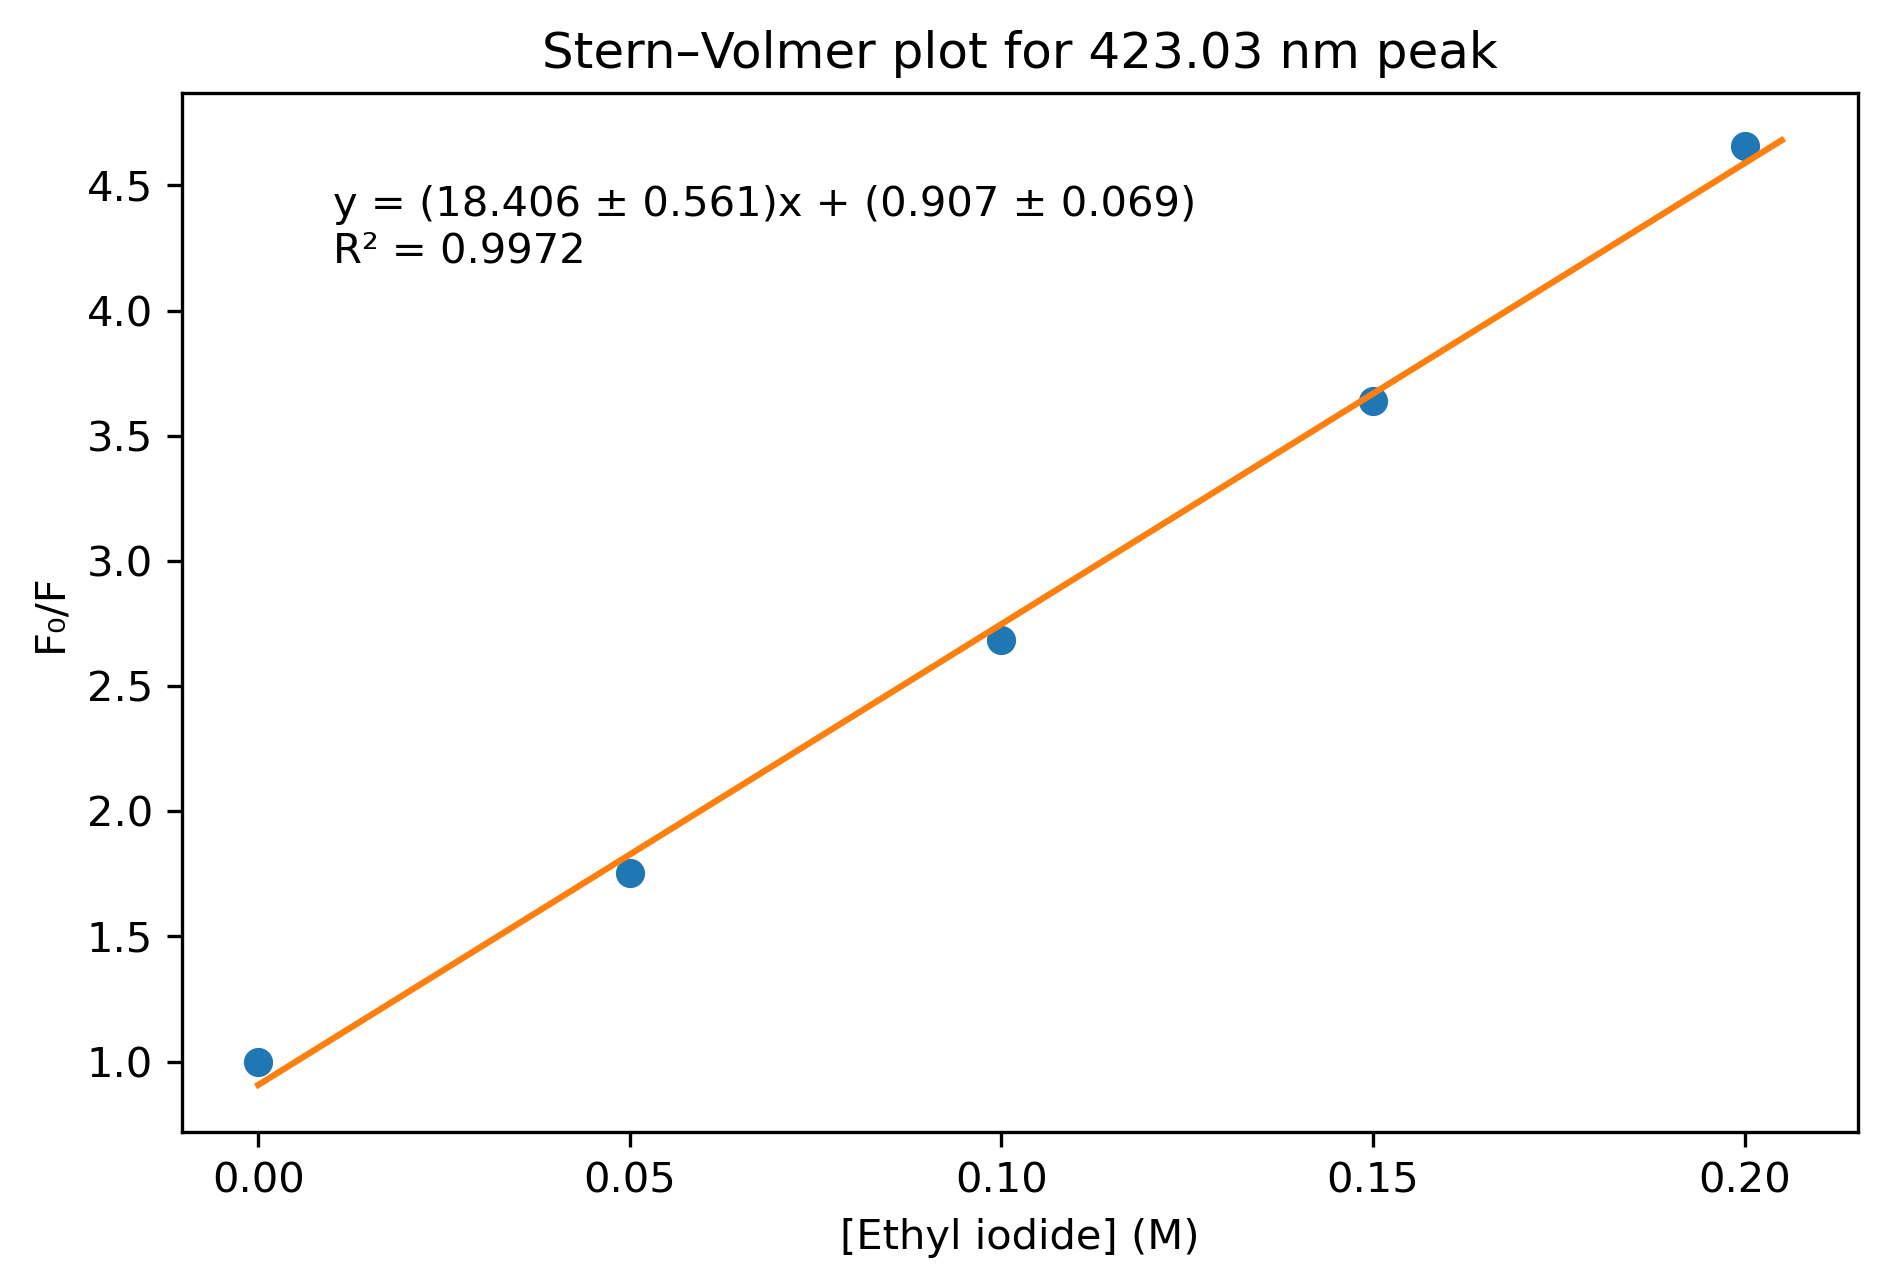
\includegraphics[width=\textwidth]{regression/stern_volmer_423p03nm.png}
        \caption{Linear Regression for Peak 3}
        \label{fig:sv_peak3}
    \end{subfigure}
    \hfill
    \begin{subfigure}[b]{0.48\textwidth}
        \centering
        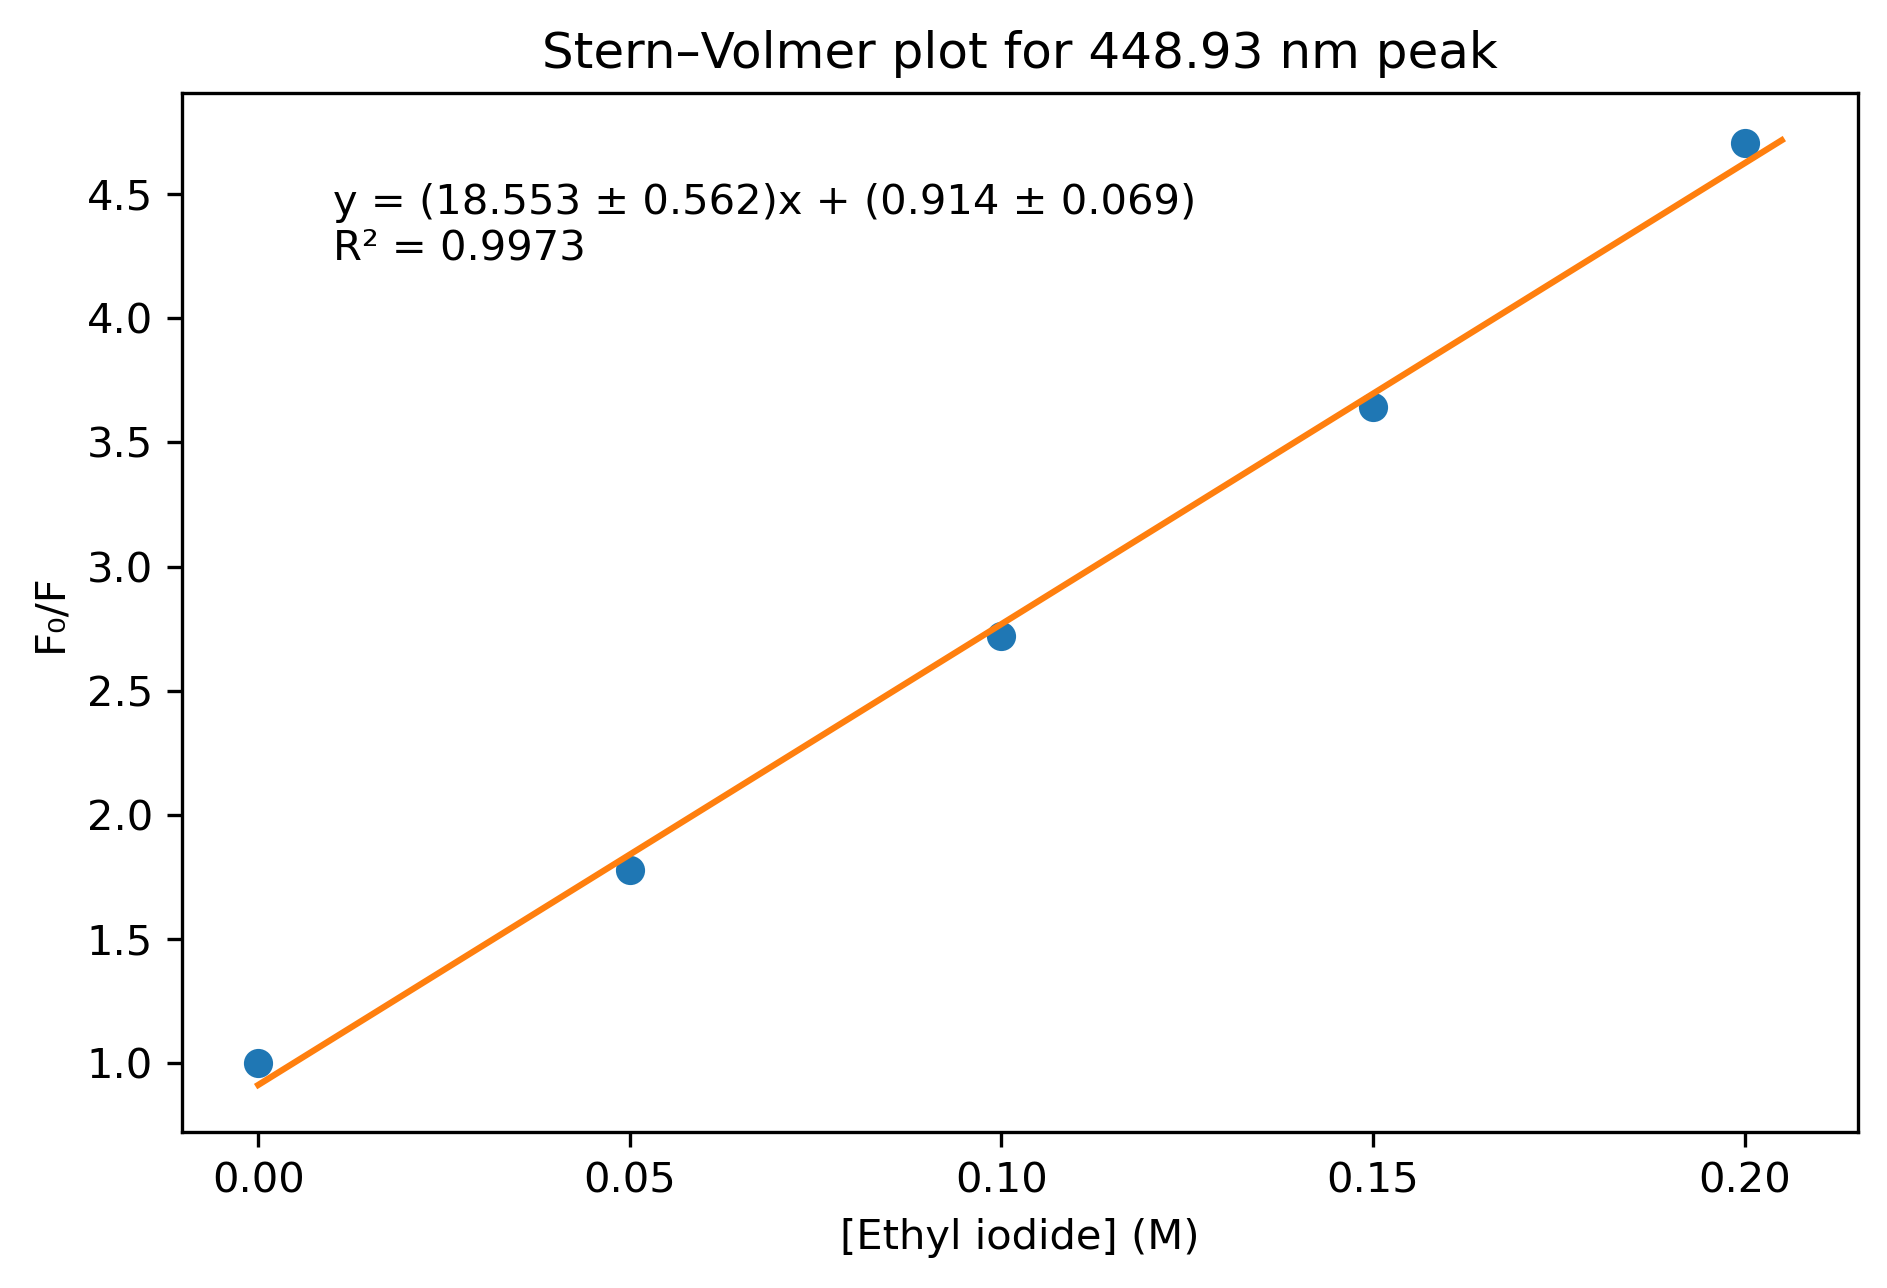
\includegraphics[width=\textwidth]{regression/stern_volmer_448p93nm.png}
        \caption{Linear Regression for Peak 4}
        \label{fig:sv_peak4}
    \end{subfigure}
    \caption{Stern-Volmer plots for the four emission peaks. Errors shown in the equations are the standard errors of the slope and intercept.}
    \label{fig:svpanel}
\end{figure}

\begin{table}[H]
\centering
\caption{Linear regression parameters for the Stern-Volmer plots.}
\label{tab:fits}
\begin{tabular}{cccccc}
\toprule
Peak / nm & Slope $k$ / M$^{-1}$ & Intercept $b$ & Standard Error($k$) / M$^{-1}$ & Standard Error($b$) & $R^2$ \\
\midrule
378.460 & 18.488 & 0.908 & 0.549 & 0.067 & 0.997 \\
399.530 & 18.551 & 0.911 & 0.532 & 0.065 & 0.998 \\
423.030 & 18.406 & 0.907 & 0.561 & 0.069 & 0.997 \\
448.930 & 18.553 & 0.914 & 0.562 & 0.069 & 0.997 \\
\bottomrule
\end{tabular}
\end{table}

The average of the four slopes was
\begin{equation}
K_{SV}^{\mathrm{exp}} = \frac{18.488+18.551+18.406+18.553}{4} = 18.500\ \mathrm{M^{-1}}
\end{equation}
The sample standard deviation of the four slopes was 0.069 M$^{-1}$, so the standard error of the mean was 0.035 M$^{-1}$. Using $t_{0.975,3}=3.182$, the 95\% confidence interval based on the spread among the four peaks was
\begin{equation}
K_{SV}^{\mathrm{exp}} = 18.500 \pm 0.110\ \mathrm{M^{-1}}
\label{eq:avgksv}
\end{equation}
This uncertainty reflects the agreement among the four fitted emission peaks rather than the regression uncertainty of any single fit.

With $\tau_0 = 4.83\times10^{-9}$ s, the apparent bimolecular quenching constant was
\begin{equation}
k_q^{\mathrm{exp}} = \frac{K_{SV}^{\mathrm{exp}}}{\tau_0}
= \frac{18.500}{4.83\times10^{-9}}
= 3.830\times10^9\ \mathrm{M^{-1}\ s^{-1}}
\end{equation}
Propagating the 95\% interval from Eq.~\ref{eq:avgksv} gives
\begin{equation}
k_q^{\mathrm{exp}} = (3.830 \pm 0.023)\times10^9\ \mathrm{M^{-1}\ s^{-1}}
\end{equation}

\section*{Discussion}
The two emission spectra recorded at 340 and 325 nm showed that the peak wavelengths changed very little, from 0.000 to 0.610 nm, while the 325 nm excitation produced a noticeably lower overall fluorescence intensity. It is consistent with Kasha's rule that, after excitation into a higher vibronic level or higher electronic state, anthracene relaxes rapidly to $S_1(v'=0)$ before emitting, so the fluorescence band positions are essentially independent of the excitation wavelength even though the detected intensity can vary with absorption efficiency and instrumental response.\cite{lab_manual}

The excitation and emission spectra both displayed regular vibronic progressions with similar spacings around 1.4 $\times 10^3$ cm$^{-1}$. The similarity is expected because excitation probes transitions from $S_0(v=0)$ to different vibronic levels of $S_1$, where fluorescence probes transitions from $S_1(v'=0)$ back to different vibronic levels of $S_0$. When the two potential energy surfaces have comparable vibrational structure, the spectra resemble one another.

Moreover, the measured excitation and emission spectra showed approximate mirror-image behavior, and the supplied reference absorption-fluorescence spectrum for anthracene in cyclohexane showed the same qualitative feature.\cite{berlman2012handbook} The symmetry was not exact, which is reasonable because solvent relaxation and the finite resolution of instrument can change the ideal behavior.

From the calculations, the $S_0$ and $S_1$ vibrational spacings are similar. The averages 1382.561 cm$^{-1}$ for $S_0$ and 1427.825 cm$^{-1}$ for $S_1$ are close on the scale of the progression. It is expected if the same skeletal vibration dominates the vibronic progression in both electronic states, though a small difference is reasonable because the excited-state force constants are not identical to those of the ground state.

From the manual\cite{lab_manual}, let the excitation rate be $R$, and let excited anthracene decay by fluorescence ($k_f$), non-radiative relaxation ($k_{nr}$), and bimolecular quenching ($k_q[Q]$). Under the steady-state approximation,
\begin{equation}
\frac{d[S_1]}{dt} = R - (k_f + k_{nr} + k_q[Q])[S_1] = 0
\end{equation}
so
\begin{equation}
[S_1] = \frac{R}{k_f + k_{nr} + k_q[Q]}
\end{equation}
Since fluorescence intensity is proportional to $k_f[S_1]$,
\begin{equation}
F \propto \frac{k_fR}{k_f + k_{nr} + k_q[Q]}
\end{equation}
and in the absence of quencher,
\begin{equation}
F_0 \propto \frac{k_fR}{k_f + k_{nr}}
\end{equation}
Therefore,
\begin{equation}
\frac{F_0}{F} = \frac{k_f + k_{nr} + k_q[Q]}{k_f + k_{nr}} = 1 + \frac{k_q[Q]}{k_f + k_{nr}}
\end{equation}
Defining the unquenched fluorescence lifetime as
\begin{equation}
\tau_0 = \frac{1}{k_f + k_{nr}}
\end{equation}
leads directly to Eq.~\ref{eq:sv}.

Comparison with literature \cite{detoma1975JACS,leite1969CPL} showed that the quenching analysis was accurate. Leite and Naqvi reported $K_1 = 18.800$ M$^{-1}$ for anthracene quenched by ethyl iodide in cyclohexane when fluorescence originates from $S_1$, while DeToma and Cowan reported $\tau_M = 4.83$ ns and $k_{TMQ} \approx 3.95\times10^9$ M$^{-1}$ s$^{-1}$, corresponding to $\tau_M k_{TMQ} \approx 19.100$ M$^{-1}$.\cite{leite1969CPL,detoma1975JACS} Relative to these two reference values, the experimental average $K_{SV}$ of 18.500 M$^{-1}$ was lower by only 1.596\% and 3.141\%, respectively. The apparent quenching constant of $3.830\times10^9$ M$^{-1}$ s$^{-1}$ was similarly close to the JACS value. 

The main limitations of the present analysis can be the finite number of data points. Nevertheless, the four regression lines were highly linear and the spread among the four peak-specific slopes was very small. Overall, the experiment supported Kasha's rule, showed near-mirror vibronic structure in excitation and fluorescence, yielding a Stern-Volmer constant well aligned with literature values.

\section*{Conclusions}
In conclusion, anthracene in cyclohexane showed well-resolved vibronic structure in both emission and excitation spectra. The fluorescence peak positions were nearly unchanged when the excitation wavelength was changed from 340 to 325 nm, consistent with Kasha's rule. Ethyl iodide quenched the fluorescence efficiently, and the Stern-Volmer analysis gave $K_{SV}=18.500 \pm 0.110 M^{-1}$ and $k_q=(3.830\pm0.023)×10^9 M^{-1} s^{-1}$ These values were in good agreement with literature results.

\bibliographystyle{unsrtnat}
\bibliography{references}

\newpage
\section*{Appendix}
\addcontentsline{toc}{section}{Appendix}
% Include supplementary material (raw output, sample calculations) 
The raw data and corresponding analysis script are available on \href{https://github.com/EasonShi0624/26Spring-PChemLab/tree/main/Lab_6_Fluorescence_of_Anthracene}{\textcolor{RoyalBlue}{GitHub} \faGithub}

\begin{figure}[htbp]
    \centering
    
\includegraphics[width=0.7\linewidth, keepaspectratio, page=1]{Lab Computation.pdf}
    \caption{Computations of Values and Error Analysis (Page 1)}
    \label{fig:lab_comp_p1}
\end{figure}

\begin{figure}[htbp]
    \centering
    
\includegraphics[width=0.9\linewidth, keepaspectratio, page=2]{Lab Computation.pdf}
    \caption{Computations of Values and Error Analysis (Page 2)}
    \label{fig:lab_comp_p1}
\end{figure}


\begin{figure}[htbp]
    \centering
    
\includegraphics[width=0.9\linewidth, keepaspectratio, page=3]{Lab Computation.pdf}
    \caption{Computations of Values and Error Analysis (Page 3)}
    \label{fig:lab_comp_p1}
\end{figure}


\begin{figure}[htbp]
    \centering
    
\includegraphics[width=0.9\linewidth, keepaspectratio, page=4]{Lab Computation.pdf}
    \caption{Computations of Values and Error Analysis (Page 4)}
    \label{fig:lab_comp_p1}
\end{figure}


\begin{figure}[htbp]
    \centering
    
\includegraphics[width=0.9\linewidth, keepaspectratio, page=5]{Lab Computation.pdf}
    \caption{Computations of Values and Error Analysis (Page 5)}
    \label{fig:lab_comp_p1}
\end{figure}

\begin{figure}[htbp]
    \centering
    
\includegraphics[width=0.9\linewidth, keepaspectratio, page=6]{Lab Computation.pdf}
    \caption{Computations of Values and Error Analysis (Page 6)}
    \label{fig:lab_comp_p1}
\end{figure}

\begin{figure}[htbp]
    \centering
    
\includegraphics[width=0.9\linewidth, keepaspectratio, page=1]{lab_note.pdf}
    \caption{Raw Lab Notes}
    \label{fig:lab_notes}
\end{figure}

\end{document}